
\documentclass[12pt]{report}
\usepackage[french]{babel}
\usepackage[utf8]{inputenc}
\usepackage{csquotes}
\usepackage[T1]{fontenc}
\usepackage{eurosym}
\usepackage{ulem}
\usepackage[a4paper,left=2.5cm,right=2.5cm,top=2.5cm,bottom=3cm]{geometry}
%\usepackage{libertine}
\usepackage{graphicx}
\usepackage{enumitem}
\usepackage{wrapfig}
\usepackage{tikz}
\usepackage{lscape}
\usepackage{multicol}
\usepackage{hyperref}
\usepackage[toc]{appendix}
\hypersetup{
    colorlinks=true,
    linkcolor=black,
    filecolor=magenta,
    urlcolor=blue,
}
\urlstyle{same}

\usepackage{tabto}

\usepackage{siunitx}
\usepackage{caption}
\usepackage{subcaption}

\usepackage{listings}
\usepackage{xcolor}

\definecolor{codegreen}{rgb}{0,0.6,0}
\definecolor{codegray}{rgb}{0.5,0.5,0.5}
\definecolor{codepurple}{rgb}{0.58,0,0.82}
\definecolor{backcolour}{rgb}{0.95,0.95,0.92}

\lstdefinestyle{mystyle}{
    backgroundcolor=\color{backcolour},   
    commentstyle=\color{codegreen},
    keywordstyle=\color{magenta},
    numberstyle=\tiny\color{codegray},
    stringstyle=\color{codepurple},
    basicstyle=\ttfamily\footnotesize,
    breakatwhitespace=false,         
    breaklines=true,                 
    captionpos=b,                    
    keepspaces=true,                 
    numbers=left,                    
    numbersep=5pt,                  
    showspaces=false,                
    showstringspaces=false,
    showtabs=false,                  
    tabsize=2
}

\lstset{style=mystyle}

\usepackage[]{biblatex}
\addbibresource{sample.bib}

\setlength{\parindent}{0cm}
\setlength{\parskip}{1ex plus 0.5ex minus 0.2ex}
\newcommand{\hsp}{\hspace{20pt}}
\newcommand{\HRule}{\rule{\linewidth}{0.5mm}}

\begin{document}

\begin{titlepage}
    \begin{sffamily}
    \begin{center}
    \Huge Can You Catch It ?
    \normalsize \\ IDASM104: Projet interdisciplinaire \\[0.5cm]

    
\includegraphics[height=9cm]{images/unamur.png}
    \\[2cm]

    
    ALBRECQ Jean, PETIT Antoine, \\ LAMBART Cyprien, DEGUELDRE Jessica
    \\[0.5cm]

    \vfill

    % Bottom of the page
    {\large Professeurs: S. Faulkner B. Frénay V. Salnikov. \\ 2020-2021}
    
    \end{center}
    \end{sffamily}
\end{titlepage}
\newpage

\tableofcontents
\newpage

\chapter{Introduction}
Le but de ce rapport est d'expliquer la démarche et la méthodologie qui a guidé l'élaboration des modèles de machine learning et de l'analyse des données fournie par les \textit{opendata stib-mivb}. Ce rapport est constitué des différentes parties: l'analyse et la préparation des données, l'entraînement des modèles de régression et de classification et l'analyse de leurs résultats. Nous nous sommes concentré uniquement sur une ligne de bus mais le système pourrait facilement être étendu au reste du réseau.

L'étape d'analyse et la préparation des données met en lumière les notions de normalisation, la détecteur d'\textit{outliers}, la selection de \textit{features}. La visualisation des données est également une partie importante de l'analyse des données. En suite dans l'étape d'entraînement des modèles passe par un phase de selection des méta-paramètres et d'optimisation des prédictions.

\section{Présentation du projet}
Il nous a été demandé de développer un nouveau service ou une analyse pertinente par rapport au défis de la mobilité. Plusieurs opendata nous était proposées, nous avons décidé de choisir celle de la STIB. Nous avons choisi de mettre en place un service permettant de savoir si prochain bus qui arrivera à un stop que l'on attend aura du retard ou non.

\chapter{Préparation et visualisation des données}

\section{Récolte des données}
La première étape est de toute évidence la récolte des données. Notre projet nous demandais d'avoir accès à un historique de retard mais malheureusement cette historique ne fait pas partie des datasets des opendata STIB. Nous avons donc développé un script python\footnote{Le code de ce script est disponible à l'adresse suivante: \href{https://github.com/jalbrecq/CanYouCatchIt/blob/main/sandbox/delay_gathering/delay_gathering.py}{lien github du script}} nous permettant de constituer cet historique de retard. Pour obtenir le délais, le script compare le temps d'arrivée théorique (qui nous est fournis par les fichiers GTFS\footnote{General Transit Feed Specification}) et l'heure d'arrivée prévue (qui nous est fournie par l'api "\textit{waiting time}"). Le délais est enregistré dans un fichier csv. En plus du délais, le script enregistre la température, la vitesse du vent, l'humidité et la visibilité grâce à l'api OpenWeather\footnote{Documentation disponible \href{https://openweathermap.org/}{ici}}. Un nouveau fichier csv est généré chaque jour.

Nous avons dans un premier temps récolté les données pour deux stop (les numéros 0089 et 6608G, voir leur emplacement dans l'annexe \ref{appendix:stop_pos_1}) du premier novembre au douze novembre. Les fichiers csv sont disponibles sur le \textit{repository}\footnote{Disponible \href{https://github.com/jalbrecq/CanYouCatchIt/tree/main/sandbox/data/csv}{ici}} du projet. Dans un second temps, nous avons récolté les données de tout les stops d'une ligne de bus (la ligne 39). La position de tout les stops de la ligne sont visible sur l'annexe \ref{appendix:stop_pos_2}\footnote{Une carte GoogleMyMaps est également disponible \href{https://www.google.com/maps/d/edit?mid=1_qNGPUfuZXrqC3UZXkmDOWuhEHJfYAox&usp=sharing}{ici}}. Les données récoltées durant cette deuxième phase sont disponible sur le \textit{repository} du projet\footnote{Disponible \href{https://github.com/jalbrecq/CanYouCatchIt/tree/main/sandbox/data/csv2}{ici}}.

\section{Premier coup d'œil à la structure des données}
La commande \lstinline!data.info()! qu'il y a 12798 lignes sans valeur pour la colonne \lstinline!delay!. Pour chacune des \textit{features} un graphique du nombre d'occurrences par valeur a été créé (voir l'annexe \ref{appendix:plots}). On peut voir sur ces graphiques que plusieurs \textit{features} ont toujours la même valeur. On peut également voir que des retards on été enregistré pour d'autres lignes que la numéro 39, il faudra donc supprimer ces dernières.

Dans le graphique en annexe \ref{appendix:plots} on remarque qu'il y a moins d'occurrences de valeur quatre pour la \textit{features} \lstinline!hour!. Cela est du au fonctionnement de l'API de la STIB. On peut également voir qu'il y a plus de d'occurrences pour les valeurs entre dix et quinze de la \textit{features} \lstinline!hour!, cette différentes est due à l'heure de démarrage et d'arrêt du script de récolte des données.

Le boxplot en annexe \ref{appendix:boxplot} montre la répartition des retards du 19 septembre sur la ligne 39 au stop 0089. On remarque que la majorité des valeurs de délais se situe entre une minute d'avance et une minute de retard.

\section{Préparation des données}

Les lignes du dataset pour les quelles la colonne \lstinline!delay! n'avait pas de valeur ont été supprimée. Les lignes dont la valeur de la colonne \lstinline!line! n'était pas égale à 39 ont également été supprimée. Les features ayant toujours la même valeur ont été supprimées. Les colonnes \lstinline!trip!, \lstinline!theoretical_time!, \lstinline!expectedArrivalTime! et \lstinline!date! ont été supprimées car elles sont pas été jugée utile. Les colonnes \lstinline!theoretical_time!, \lstinline!expectedArrivalTime! et \lstinline!date! ont été supprimées car les valeurs étaient du type \lstinline!string!. La colonne \lstinline!date! a été considérée comme redondante, sa valeur étant déjà stockée dans les colonnes \lstinline!hour!, \lstinline!minute! et \lstinline!day!.

\subsection{Stratification des données}
La stratification des données ne nous a pas semblé utile car le dataset n'est assez grand pour rendre cette dernière nécessaire. Cependant dans un but pédagogique nous avons quand même stratifier la colonne \lstinline!hour!, afin que la répartition des différentes valeurs reste identique dans le dataset ainsi que dans le test-set.

\section{Visualisation des données}
\subsection{Création du test-set}
Cela pourrait paraître étrange de mettre de coté une partie des données à ce moment. Les données n'ont même pas encore été vraiment visualisée et nous devons encore en apprendre plus avant de choisir quel algorithmes utiliser. Cependant si le test-set est créé maintenant c'est pour éviter le \textit{snooping bias}. Le test-set et constituer de vingt pourcent des données du dataset. 

\subsection{Création des visualisations}
La première visualisation générée (annexe \ref{appendix:delay_per_hour}) est la répartition des délais en fonction de l'heure. On remarque qu'après dix-huit heure on a soit une avance ou un retard de vingt minutes ou une variation de cinq minutes par rapport à l'horaire théorique, sans valeur intermédiaire. On remarque également que la majorité des délais ont une valeur nulle. On peut également voir qu'il une augmentation des délais après quinze heure jusqu'a dix-neuf heure.

Le second graphique (annexe \ref{appendix:mean_delay_per_hour}) indique le délais moyen par heure. On y remarque une augmentation des délais entre six et neuf heure, à quinze heure et ainsi qu'a vingt-et-une heure. Le pick de retard de vingt-et-une heure vient sans doute du couvre feu de vingt-deux heure, les autres pick quand à eux sont à priori du au traffic de Bruxelles.

Sur la dernière infographie (annexe \ref{appendix:mean_temp_per_hour}) on remarque une hausse des températures de midi à seize heure.

\begin{appendices}
    \chapter{Position des stops}
    \begin{figure}[h]
        \centering
        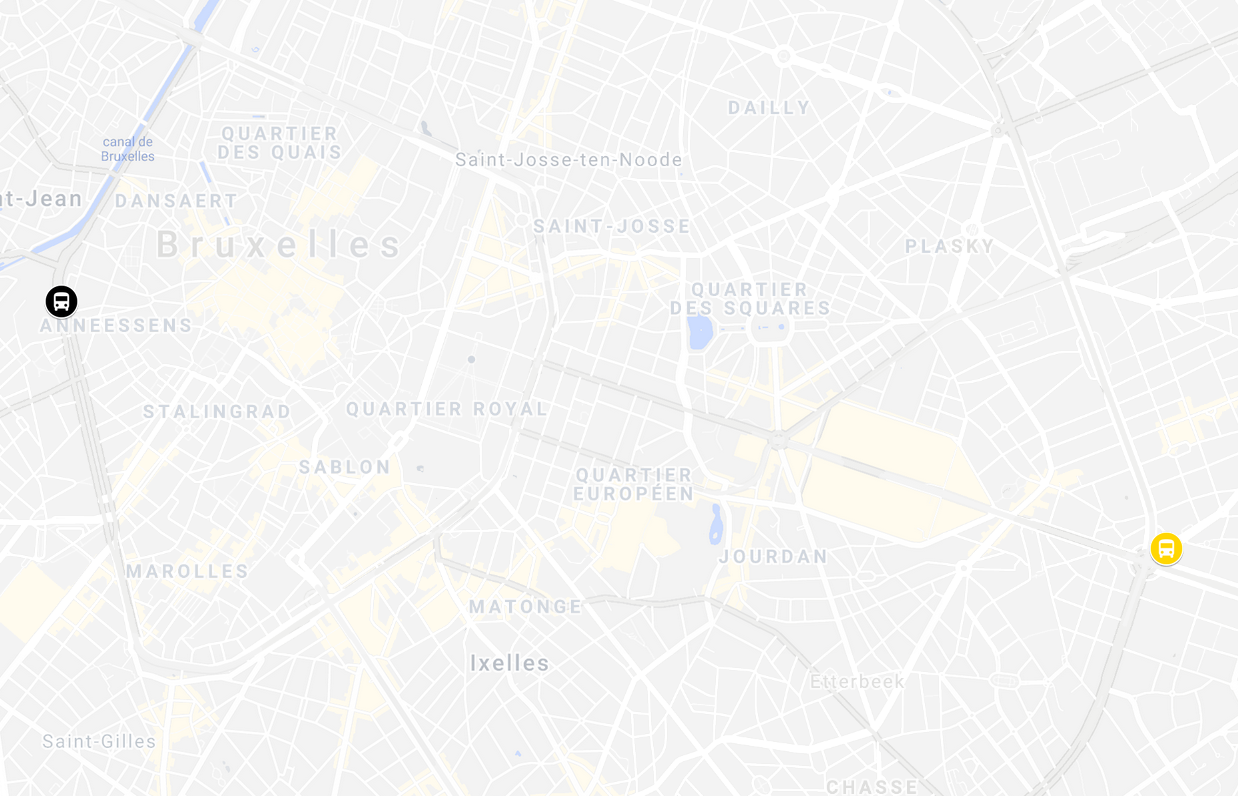
\includegraphics[width=0.7\textwidth]{images/stop_pos_1.png}
        \caption{Position des stops numéro 0089 et 6608G en jaune et noir respectivement.}
        \label{appendix:stop_pos_1}
    \end{figure}

    \begin{figure}[h]
        \centering
        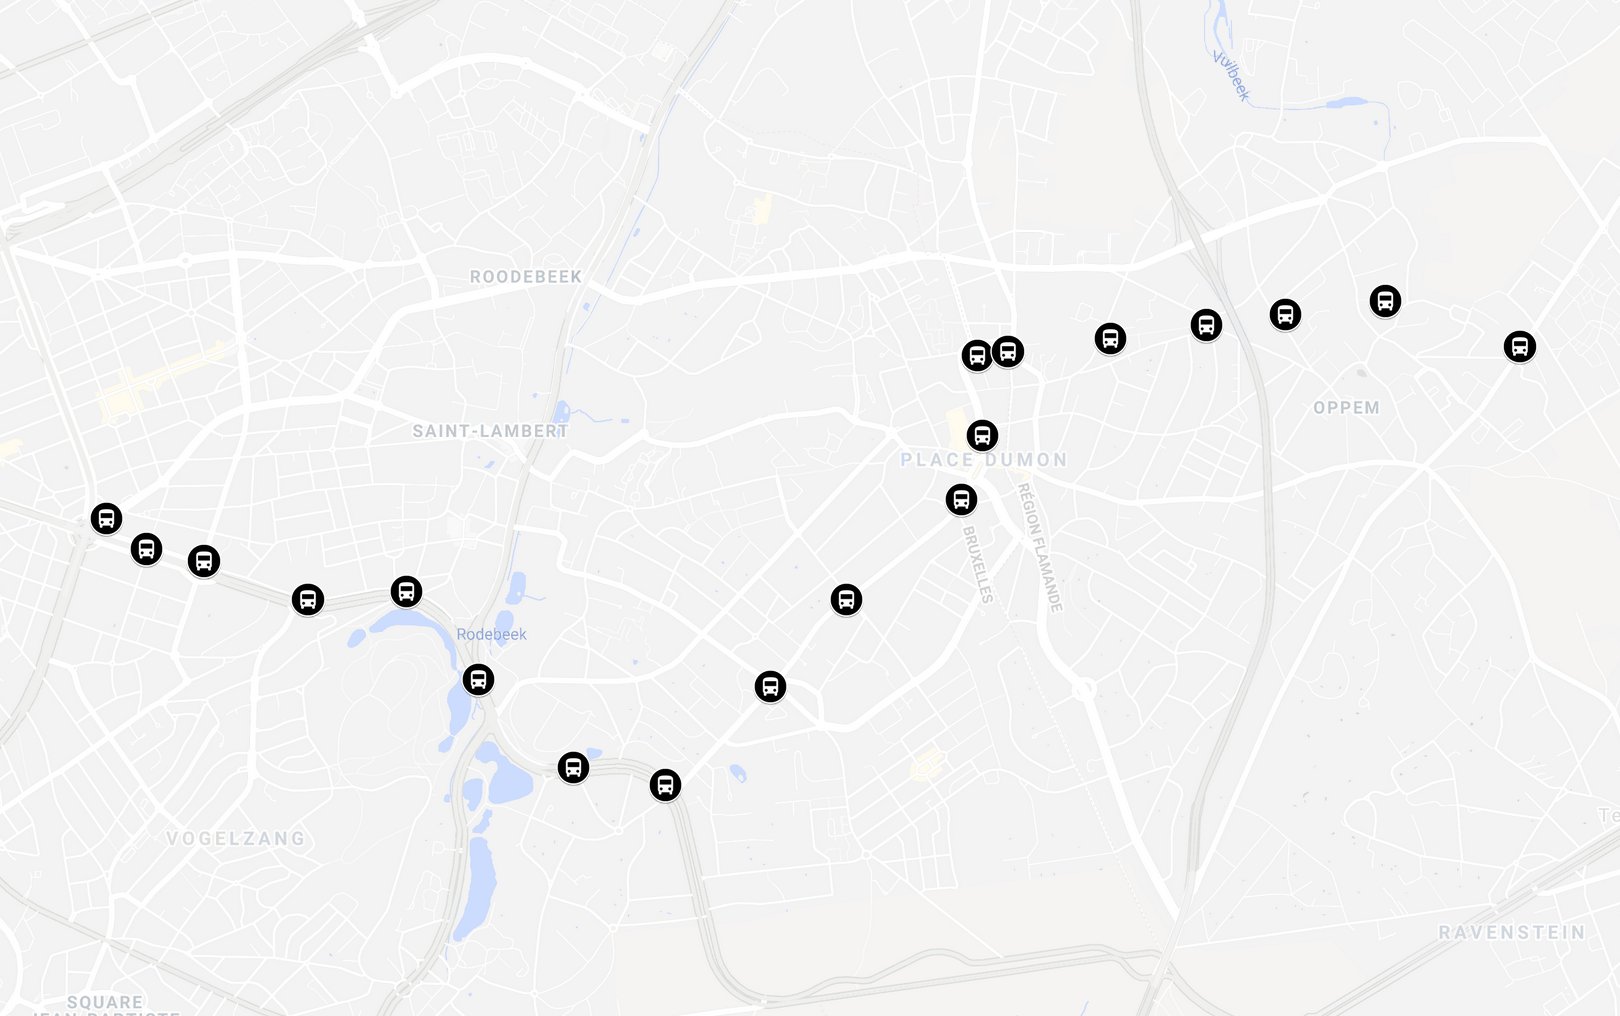
\includegraphics[width=0.7\textwidth]{images/stop_pos_2.png}
        \caption{Position des stops présent sur la ligne 39}
        \label{appendix:stop_pos_2}
    \end{figure}

    \chapter{Première visualisation des données}
    \begin{figure}[h]
        \centering
        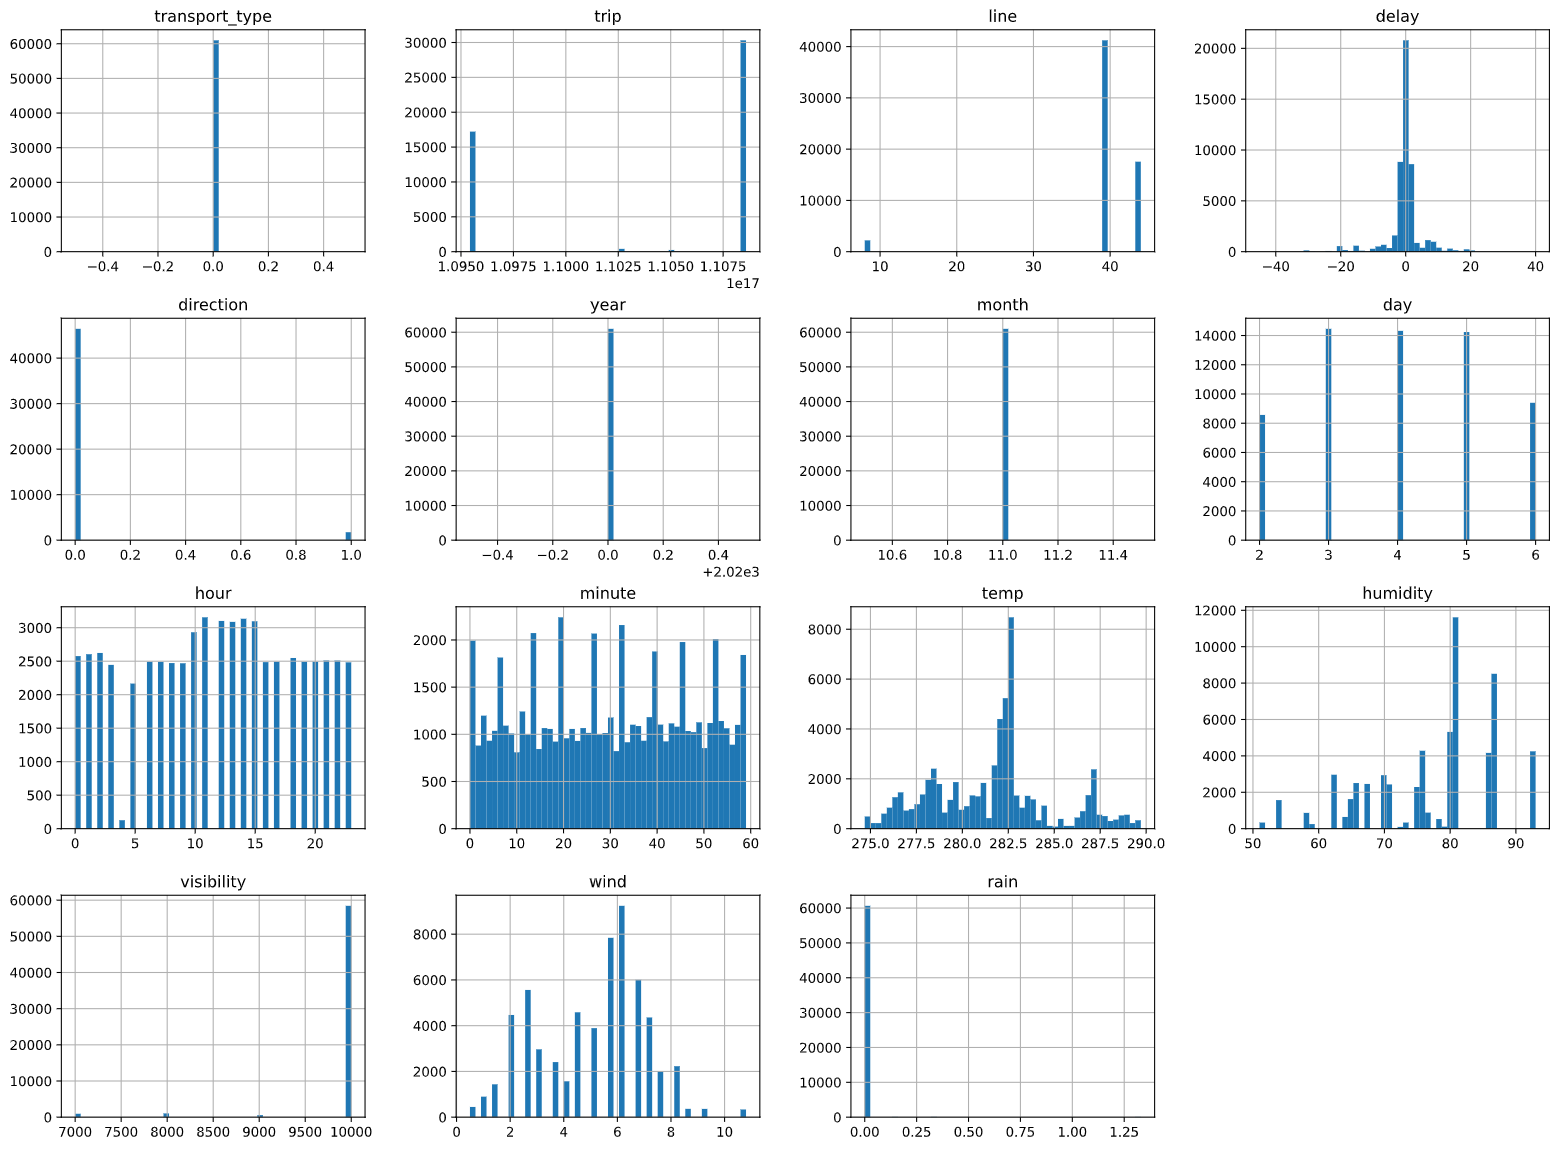
\includegraphics[width=0.7\textwidth]{images/plots.png}
        \caption{Plot des features par nombre d'occurrences}
        \label{appendix:plots}
    \end{figure}

    \begin{figure}[h]
        \centering
        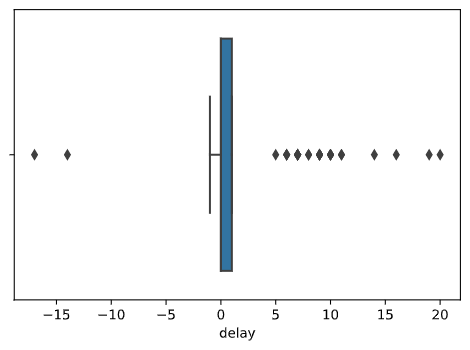
\includegraphics[width=0.7\textwidth]{images/boxplot.png}
        \caption{Boxplot des délais du 19 septembre sur la ligne 39 au stop 0089}
        \label{appendix:boxplot}
    \end{figure}

    \begin{figure}[h]
        \centering
        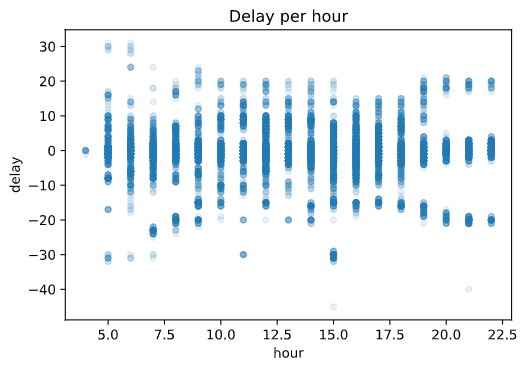
\includegraphics[width=0.7\textwidth]{images/delay_per_hour.png}
        \caption{Délai par heure pour tout le dataset}
        \label{appendix:delay_per_hour}
    \end{figure}

    \begin{figure}[h]
        \centering
        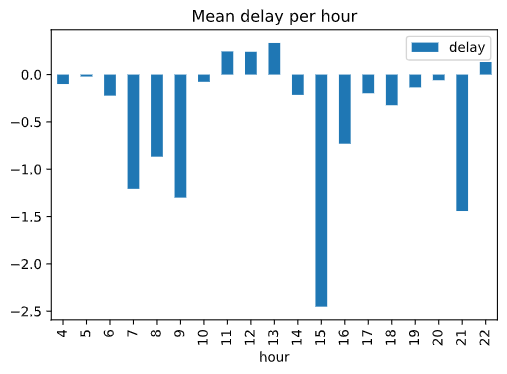
\includegraphics[width=0.7\textwidth]{images/mean_delay_per_hour.png}
        \caption{Délai moyen par heure pour tout le dataset}
        \label{appendix:mean_delay_per_hour}
    \end{figure}

    \begin{figure}[h]
        \centering
        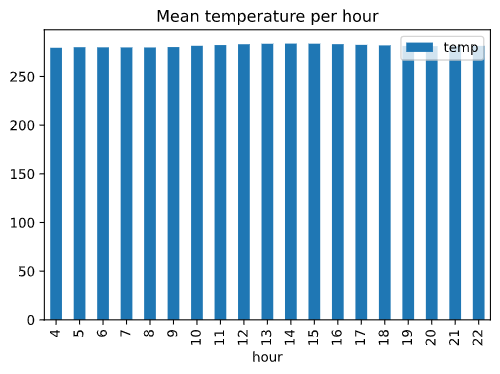
\includegraphics[width=0.7\textwidth]{images/mean_temp_per_hour.png}
        \caption{Température moyenne par heure pour tout le dataset}
        \label{appendix:mean_temp_per_hour}
    \end{figure}

\end{appendices}

\lstlistoflistings

\nocite{*}
\printbibliography
\end{document}
